% Options for packages loaded elsewhere
\PassOptionsToPackage{unicode}{hyperref}
\PassOptionsToPackage{hyphens}{url}
%
\documentclass[
  man,floatsintext]{apa6}
\usepackage{amsmath,amssymb}
\usepackage{iftex}
\ifPDFTeX
  \usepackage[T1]{fontenc}
  \usepackage[utf8]{inputenc}
  \usepackage{textcomp} % provide euro and other symbols
\else % if luatex or xetex
  \usepackage{unicode-math} % this also loads fontspec
  \defaultfontfeatures{Scale=MatchLowercase}
  \defaultfontfeatures[\rmfamily]{Ligatures=TeX,Scale=1}
\fi
\usepackage{lmodern}
\ifPDFTeX\else
  % xetex/luatex font selection
\fi
% Use upquote if available, for straight quotes in verbatim environments
\IfFileExists{upquote.sty}{\usepackage{upquote}}{}
\IfFileExists{microtype.sty}{% use microtype if available
  \usepackage[]{microtype}
  \UseMicrotypeSet[protrusion]{basicmath} % disable protrusion for tt fonts
}{}
\makeatletter
\@ifundefined{KOMAClassName}{% if non-KOMA class
  \IfFileExists{parskip.sty}{%
    \usepackage{parskip}
  }{% else
    \setlength{\parindent}{0pt}
    \setlength{\parskip}{6pt plus 2pt minus 1pt}}
}{% if KOMA class
  \KOMAoptions{parskip=half}}
\makeatother
\usepackage{xcolor}
\usepackage{graphicx}
\makeatletter
\def\maxwidth{\ifdim\Gin@nat@width>\linewidth\linewidth\else\Gin@nat@width\fi}
\def\maxheight{\ifdim\Gin@nat@height>\textheight\textheight\else\Gin@nat@height\fi}
\makeatother
% Scale images if necessary, so that they will not overflow the page
% margins by default, and it is still possible to overwrite the defaults
% using explicit options in \includegraphics[width, height, ...]{}
\setkeys{Gin}{width=\maxwidth,height=\maxheight,keepaspectratio}
% Set default figure placement to htbp
\makeatletter
\def\fps@figure{htbp}
\makeatother
\setlength{\emergencystretch}{3em} % prevent overfull lines
\providecommand{\tightlist}{%
  \setlength{\itemsep}{0pt}\setlength{\parskip}{0pt}}
\setcounter{secnumdepth}{-\maxdimen} % remove section numbering
% Make \paragraph and \subparagraph free-standing
\ifx\paragraph\undefined\else
  \let\oldparagraph\paragraph
  \renewcommand{\paragraph}[1]{\oldparagraph{#1}\mbox{}}
\fi
\ifx\subparagraph\undefined\else
  \let\oldsubparagraph\subparagraph
  \renewcommand{\subparagraph}[1]{\oldsubparagraph{#1}\mbox{}}
\fi
\ifLuaTeX
\usepackage[bidi=basic]{babel}
\else
\usepackage[bidi=default]{babel}
\fi
\babelprovide[main,import]{english}
% get rid of language-specific shorthands (see #6817):
\let\LanguageShortHands\languageshorthands
\def\languageshorthands#1{}
% Manuscript styling
\usepackage{upgreek}
\captionsetup{font=singlespacing,justification=justified}

% Table formatting
\usepackage{longtable}
\usepackage{lscape}
% \usepackage[counterclockwise]{rotating}   % Landscape page setup for large tables
\usepackage{multirow}		% Table styling
\usepackage{tabularx}		% Control Column width
\usepackage[flushleft]{threeparttable}	% Allows for three part tables with a specified notes section
\usepackage{threeparttablex}            % Lets threeparttable work with longtable

% Create new environments so endfloat can handle them
% \newenvironment{ltable}
%   {\begin{landscape}\centering\begin{threeparttable}}
%   {\end{threeparttable}\end{landscape}}
\newenvironment{lltable}{\begin{landscape}\centering\begin{ThreePartTable}}{\end{ThreePartTable}\end{landscape}}

% Enables adjusting longtable caption width to table width
% Solution found at http://golatex.de/longtable-mit-caption-so-breit-wie-die-tabelle-t15767.html
\makeatletter
\newcommand\LastLTentrywidth{1em}
\newlength\longtablewidth
\setlength{\longtablewidth}{1in}
\newcommand{\getlongtablewidth}{\begingroup \ifcsname LT@\roman{LT@tables}\endcsname \global\longtablewidth=0pt \renewcommand{\LT@entry}[2]{\global\advance\longtablewidth by ##2\relax\gdef\LastLTentrywidth{##2}}\@nameuse{LT@\roman{LT@tables}} \fi \endgroup}

% \setlength{\parindent}{0.5in}
% \setlength{\parskip}{0pt plus 0pt minus 0pt}

% Overwrite redefinition of paragraph and subparagraph by the default LaTeX template
% See https://github.com/crsh/papaja/issues/292
\makeatletter
\renewcommand{\paragraph}{\@startsection{paragraph}{4}{\parindent}%
  {0\baselineskip \@plus 0.2ex \@minus 0.2ex}%
  {-1em}%
  {\normalfont\normalsize\bfseries\itshape\typesectitle}}

\renewcommand{\subparagraph}[1]{\@startsection{subparagraph}{5}{1em}%
  {0\baselineskip \@plus 0.2ex \@minus 0.2ex}%
  {-\z@\relax}%
  {\normalfont\normalsize\itshape\hspace{\parindent}{#1}\textit{\addperi}}{\relax}}
\makeatother

\makeatletter
\usepackage{etoolbox}
\patchcmd{\maketitle}
  {\section{\normalfont\normalsize\abstractname}}
  {\section*{\normalfont\normalsize\abstractname}}
  {}{\typeout{Failed to patch abstract.}}
\patchcmd{\maketitle}
  {\section{\protect\normalfont{\@title}}}
  {\section*{\protect\normalfont{\@title}}}
  {}{\typeout{Failed to patch title.}}
\makeatother

\usepackage{xpatch}
\makeatletter
\xapptocmd\appendix
  {\xapptocmd\section
    {\addcontentsline{toc}{section}{\appendixname\ifoneappendix\else~\theappendix\fi\\: #1}}
    {}{\InnerPatchFailed}%
  }
{}{\PatchFailed}
\keywords{keywords\newline\indent Word count: X}
\usepackage{csquotes}
\ifLuaTeX
  \usepackage{selnolig}  % disable illegal ligatures
\fi
\IfFileExists{bookmark.sty}{\usepackage{bookmark}}{\usepackage{hyperref}}
\IfFileExists{xurl.sty}{\usepackage{xurl}}{} % add URL line breaks if available
\urlstyle{same}
\hypersetup{
  pdftitle={Memory specificity in evaluation conditioning: a `Who said what' approach},
  pdfauthor={Jéréline Benading1 \& Klaus Rothermund2},
  pdflang={en-EN},
  pdfkeywords={keywords},
  hidelinks,
  pdfcreator={LaTeX via pandoc}}

\title{Memory specificity in evaluation conditioning: a `Who said what' approach}
\author{Jéréline Benading\textsuperscript{1} \& Klaus Rothermund\textsuperscript{2}}
\date{}


\shorttitle{Memory specificity in EC}

\authornote{

Correspondence concerning this article should be addressed to Jéréline Benading, . E-mail: \href{mailto:karoline.bading@uni-jena.de}{\nolinkurl{karoline.bading@uni-jena.de}}

}

\affiliation{\vspace{0.5cm}\textsuperscript{1} Université Agnostique de Louvain-la-Jena\\\textsuperscript{2} Friedrich Schiller University Jena}

\abstract{%
BLABLABLABLABLA
}



\begin{document}
\maketitle

Please insert: introduction leading up to one the greatest studies of all time.

\hypertarget{amazing-paraphraph}{%
\subsection{Amazing paraphraph}\label{amazing-paraphraph}}

Please insert: a great paragraph

\hypertarget{another-amazing-paraphraph}{%
\subsection{Another amazing paraphraph}\label{another-amazing-paraphraph}}

Please insert: a great paragraph

\hypertarget{methods}{%
\section{Methods}\label{methods}}

We report how we determined our sample size, all data exclusions, all manipulations, and all measures. The preregistration, experiment program, data, and analyses are publicly available on the Open Science Framework at: \url{https://osf.io/rqkvy/}.

The study project was approved by the ethics committee of \emph{{[}Institution Redacted{]}} (\emph{{[}ID Redacted{]}}).

\hypertarget{participants-and-design}{%
\subsection{Participants and design}\label{participants-and-design}}

The experiment used a 2 (US valence: Positive vs.~Negative vs.~None) x 2 (Task order: Evaluation first vs.~Memory first) mixed design, with US valence manipulated within participants and Task order manipulated between participants.

We recruited 172 participants (50\(\%\) female; \(M_{age} =\) 39.59; \(SD_{age} =\) 13.23), our targeted sample size, online on Prolific. Participants were English speakers, had an approval rate of at least 90\% and at least 100 previous submissions, and did not take part in previous evaluative conditioning studies we conducted on Prolific. Data were unavailable for one participant, and we excluded 5 participants declaring that they did not pay attention or did not take their responses seriously. This resulted in a final sample size of 166 participants (\(n =\) 70 in the Evaluation first condition and \(n =\) 96 in the Memory first condition).

To determine sample size, we set \(\alpha\) to .05, and we aimed for a statistical power of at least \(80\%\) to detect an Evaluative Conditioning effect as small as Cohen's \(d = 0.2\) in a one-sided paired sample \emph{t}-test (IV: US valence; DV: evaluative ratings). An analysis with the R package \emph{pwr} (version 1.3-0; Champely, 2020) showed that we needed 156 participants. A sample size of \emph{N} = 156 also provided \(80%
\) power to detect correlations \(rs \geq .22\) (e.g., between parameter estimates and evaluative conditioning scores). To avoid a final sample smaller than the targeted sample size after applying the exclusion criteria, we increased this estimate by 10\%, resulting in 172 participants.

\hypertarget{materials-and-procedure}{%
\subsection{Materials and procedure}\label{materials-and-procedure}}

We programmed the experiment with lab.js (Henninger et al., 2022). We exported the study to an HTTPS-protected website with JATOS (Lange et al., 2015).

\hypertarget{stimuli}{%
\subsubsection{Stimuli}\label{stimuli}}

As neutral stimuli, we used 54 5- to 7-letter nonwords (all made of a combination of vowels and consonants; e.g., `\emph{botsy}'; `\emph{ampfong}') used in a previous study (Stahl \& Bading, 2020). On a participant basis, 24 nonwords were used as CSs (paired with USs in the learning phase) and 24 were new (i.e., presented only in the test phase).

The USs were 24 color images of animals (e.g., a cockroach), scenes (e.g., a rainbow), and objects (e.g., a knife) selected from the Open Affective Standardized Image Set (OASIS; Kurdi et al., 2017). Based on OASIS ratings (on a 7-point Likert scale), twelve images were positive (\(M_{valence} = 5.88\); \(SD_{valence}\) = 0.24; \(M_{arousal} = 4.10\); \(SD_{arousal} = 0.50\)) and 12 were negative (\(M_{valence} = 2.05\); \(SD_{valence} = 0.32\); \(M_{arousal} = 4.27\); \(SD_{arousal} = 0.52\)). Positive USs were significantly more positive than negative USs, Welch's \(t(20.23) = 33.36, p < .001\). Positive and negative USs did not significantly differ in arousal, Welch's \(t(21.96) = 0.82, p = .419\).

\hypertarget{learning-phase}{%
\subsubsection{Learning phase}\label{learning-phase}}

After providing their informed consent, participants entered the learning phase. Participants were told that they would see pairs made of one nonword (the CSs; on the center-left of the screen) and one image (the USs on the center-right of the screen). Participants had to pay close attention to each pair.

Twenty-four CS-US pairs were presented three times each in a random order (block-wise) for 1000 milliseconds (separated by an inter-trial interval of 1000 ms), resulting in 72 trials. For each participant, the 24 CSs were randomly drawn from the pool of 54 nonwords. Each CS was paired with one specific US. The CSs were displayed in a sans-serif font (font-size: 40). The dimensions of the USs were 250 pixels (width) and 200 pixels (height).

\hypertarget{test-phase}{%
\subsubsection{Test phase}\label{test-phase}}

After the learning phase, participants entered the test phase. Participants performed two tasks: an evaluative rating task and a memory task. Participants were randomly assigned to one of the two Task order conditions. In the Evaluation first condition, participants performed the evaluative rating task and then the memory task. The order was reversed in the Memory first condition: participants performed the memory task and then the evaluative rating task. The exact wording of the tasks slightly differed as a function of Task order.

\hypertarget{evaluative-rating-task}{%
\paragraph{Evaluative rating task}\label{evaluative-rating-task}}

In the evaluative classification task, the 24 CSs presented in the learning phase and 24 new nonwords (randomly drawn from the remaining pool of 30 nonwords) were displayed individually once in a random order without time limit. Participants rated how positive or negative they found the nonwords on a 8-point Likert scale ranging from 1 ``very negative'' to 8 ``very positive.'' The 48 trials were separated by 500-ms inter-trial intervals.

\hypertarget{memory-task}{%
\paragraph{Memory task}\label{memory-task}}

In the memory task, the 24 CSs presented in the learning phase and 24 new nonwords (identical to the ones displayed in the evaluative rating task) were displayed individually once in a random order without time limit.

Each of the trials began with a recognition memory task. Participants were asked whether the nonwords were part of the pairs presented in the learning phase (response options: ``Yes (old)''; ``No (new)'').

If participants responded ``No (new),'' the next recognition memory trial began after a 500-ms inter-trial interval. If participants responded ``Yes (old),'' a new screen including the same nonword appeared after a 500-ms blank screen, and participants had to select the specific image that the nonword was paired with. Participants were instructed to click on the specific image if they remembered it or to guess the correct image if they could not remember the exact image. Eight images (all from the learning phase) were displayed in two rows of four images. For nonwords that were correctly recognized (hits), the correct US was presented with 7 randomly selected distractors (3 images of the same valence as the correct US; 4 images of the opposite valence). All the USs were allocated to a random position. For nonwords that were incorrectly recognized (false alarms), 8 USs, half positive and half negative, were randomly selected and allocated to a random position.

\hypertarget{check-measures}{%
\paragraph{Check measures}\label{check-measures}}

After the test phase, we administered an attention check and a seriousness check. In the attention check, we asked participants whether they paid attention to the nonwords and images presented throughout the study (Yes/No response). Participants were told that their response would not affect their payment.

In the seriousness check based on Aust et al.~(2013), participants read:

\emph{``It would be very helpful if you could tell us at this point whether you have taken the requested responses seriously, so that we can use your answers for our scientific analysis, or whether you were just clicking through to take a look at the survey? (again, this will not affect your payment).''}

The response options were \emph{``I have taken the requested responses seriously''} and \emph{``I have just clicked through, please discard my data''}. We used the answers to the attention and seriousness checks as exclusion criteria (see the Participants and design section).

Participants then had the chance to comment on the study. Finally, participants were thanked and debriefed.

\hypertarget{data-processing-and-analyses}{%
\subsection{Data processing and analyses}\label{data-processing-and-analyses}}

BLABLABLA

\hypertarget{results}{%
\section[Results]{\texorpdfstring{Results\footnote{All analyses were conducted with R (R Core Team, 2021). We used the packages XXX (), XXX (), XXX (), XXX (), XXX (), XXX (), XXX ()\ldots{}}}{Results}}\label{results}}

\hypertarget{preregistered-analyses-on-evaluative-ratings}{%
\subsection{Preregistered analyses on evaluative ratings}\label{preregistered-analyses-on-evaluative-ratings}}

We report the analyses we conducted on evaluative ratings. We averaged evaluative ratings as a function of US valence (Positive, Negative, None) and Task order (Evaluation first, Memory first). For each participant, we calculated an Evaluative Conditioning (EC) score, which is their mean evaluative rating on CSs paired with positive USs minus their mean evaluative rating on CSs paired with negative USs (negative scores indicate higher evaluations on negatively paired vs.~positively paired CSs; positive scores indicate higher evaluations on positively vs.~negatively paired CSs).

First, we conducted a between-participants ANOVA on EC scores with Task order as the only factor. We tested whether the grand mean was above 0 by calculating the F-test of the intercept. A grand mean above 0 would indicate that, overall, we replicated the EC effect. In line with the preregistration, we divided the \emph{p}-value of this test by two to perform a one-tailed test, as the grand mean of EC scores was above 0 (\(M =\) 0.72; \(SD =\) 0.97). The \emph{F}-test was significant, \(F(1, 164) = 92.25\), \(p < .001\), \(\hat{\eta}^2_G = .360\), 90\% CI \([.267, .444]\), showing that we replicated the EC effect. The effect of Task order was not significant\footnote{As preregistered, we divided the \emph{p}-value by two to perform a one-tailed version of the test (similar to \emph{t}-tests) because EC scores are descriptively larger in the Evaluation first (\(M =\) 0.80; \(SD =\) 0.87) than Memory first (\(M =\) 0.66; \(SD =\) 1.03) condition. EC scores were above 0 both in the Evaluation first condition, \(t(69) = 7.76\), \(p < .001\), \(d =\) 0.93, 90\% CI = {[}0.69, 1.16{]} and in the Memory first condition, \(t(95) = 6.22\), \(p < .001\), \(d =\) 0.63, 90\% CI = {[}0.45, 0.82{]}.}, \(F(1, 164) = 0.94\), \(p = .334\), \(\hat{\eta}^2_G = .006\), 90\% CI \([.000, .040]\), which means that performing the evaluative rating task before or after the memory task did not significantly change the EC effect.

\begin{figure}
\centering
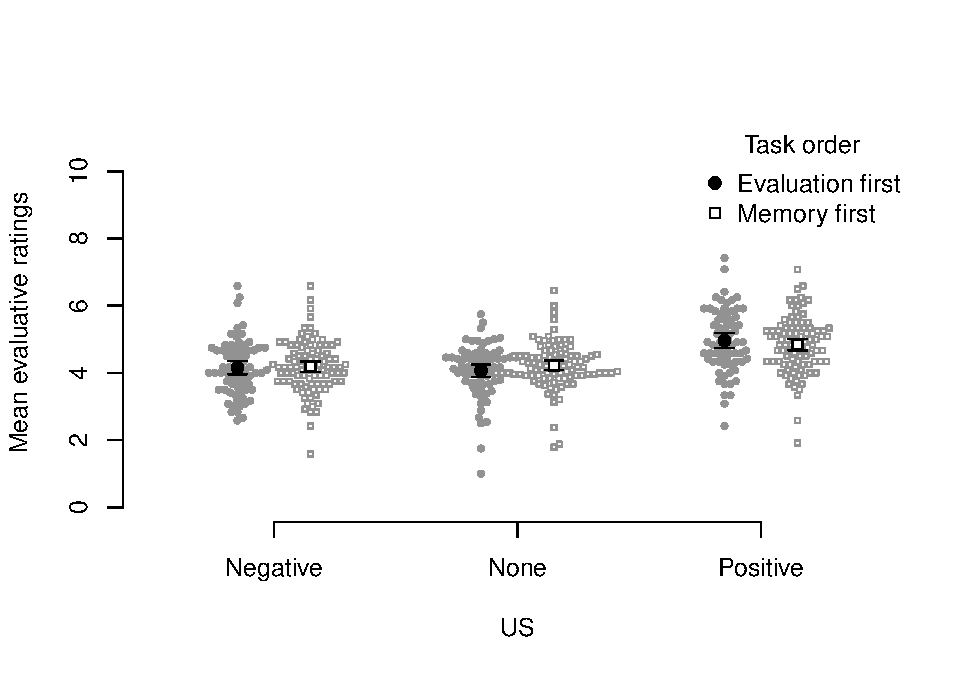
\includegraphics{main_files/figure-latex/plot_us_valence_order-1.pdf}
\caption{(\#fig:plot\_us\_valence\_order)Mean evaluative ratings (and 95\% error bars) as a function of US valence and Task order.}
\end{figure}

Complementarily, we also conducted a 3 (US valence) x 2 (Task order) mixed ANOVA on evaluative ratings (see Figure @ref(fig:plot\_us\_valence\_order)). Different from the ANOVA above, evaluative ratings on unpaired nonwords can be compared with evaluations in other conditions. The main effect of US valence was significant, \(F(2, 328) = 68.83\), \(p < .001\), \(\hat{\eta}^2_G = .156\), 90\% CI \([.099, .214]\). We followed-up on the ANOVA by conducting multiple comparisons (Bonferroni-corrected) based on the full model: evaluative ratings were higher for positively paired CSs compared with new non-words, \(t(164) = -9.94, p < .001, d = 0.75, 95\%\) CI \(= [0.58, 0.92]\), and compared with negatively-paired CSs, \(t(164) = -9.61, p < .001, d = 0.74, 95\%\) CI \(= [0.57, 0.91]\). Evaluative ratings were not significantly different for negatively-paired CSs and for nonwords, \(t(164) = -0.39, p = .922, d = 0.02, 95\%\) CI \(= [-0.13, 0.17]\). The main effect of Task order was not significant, \(F(1, 164) = 0.04\), \(p = .844\), \(\hat{\eta}^2_G = .000\), 90\% CI \([.000, .010]\), nor was the interaction between US valence and Task order, \(F(2, 328) = 1.81\), \(p = .166\), \(\hat{\eta}^2_G = .005\), 90\% CI \([.000, .021]\).

\hypertarget{preregistered-analyses-on-memory-performance}{%
\subsection{Preregistered analyses on memory performance}\label{preregistered-analyses-on-memory-performance}}

XXX

\hypertarget{preregistered-analyses-on-evaluations-as-a-function-of-mpt-parameter-estimates}{%
\subsection{Preregistered analyses on evaluations as a function of MPT parameter estimates}\label{preregistered-analyses-on-evaluations-as-a-function-of-mpt-parameter-estimates}}

XXX

\hypertarget{mpt-model}{%
\subsection{MPT model}\label{mpt-model}}

Amazing result 2

\hypertarget{relationships-between-ratings-and-parameters}{%
\subsection{Relationships between ratings and parameters}\label{relationships-between-ratings-and-parameters}}

Amazing result 3

\hypertarget{general-discussion}{%
\section{General discussion}\label{general-discussion}}

\hypertarget{amazing-paragraph}{%
\subsection{Amazing paragraph}\label{amazing-paragraph}}

smart conclusion 1

\hypertarget{another-amazing-paragraph}{%
\subsection{Another amazing paragraph}\label{another-amazing-paragraph}}

smart conclusion 2

\hypertarget{appendix}{%
\section{Appendix}\label{appendix}}

\hypertarget{appendix-appendix}{%
\appendix}


\hypertarget{amazing-paragraph-1}{%
\subsection{Amazing paragraph}\label{amazing-paragraph-1}}

additional information on something amazing

\hypertarget{another-amazing-paragraph-1}{%
\subsection{Another amazing paragraph}\label{another-amazing-paragraph-1}}

more information on another amazing thing


\end{document}
